\documentclass[conference]{IEEEtran}
\IEEEoverridecommandlockouts
\usepackage{cite,amsmath,amssymb,graphicx,booktabs,url}
\usepackage{tikz}
\usetikzlibrary{arrows.meta,positioning,fit,backgrounds}
\usepackage[colorlinks=true,linkcolor=black,citecolor=black,urlcolor=blue]{hyperref}

% Allow IEEE's narrow columns to break long prose and bibliography entries cleanly.
\setlength{\emergencystretch}{3em}

\begin{document}

\title{When Does Stigmergic Routing Help Evacuation?\\[2pt]
\large An Empirical Study of Dynamic Ant Colony Optimization under Spreading Fire,\\
Partial Observability, and Compute Budgets}

\author{\IEEEauthorblockN{Sathvika R.} % Verify author name before submission
\IEEEauthorblockA{\textit{Independent Researcher}\\
Bengaluru, India\\
\href{https://github.com/Sathvikar01}{\texttt{github.com/Sathvikar01}}}}

\maketitle

\begin{abstract}
Six policy implementations---random walk, greedy BFS-distance, per-tick hazard-aware A*, incremental D* Lite, Standard ACO, and Full CMS-DACO---are evaluated across matched seeded environments. We use paired t-tests, Wilcoxon signed-rank tests, paired bootstrap confidence intervals, and Holm correction. Results show that hazard-aware A* remains the strongest policy on the tested small-to-medium maps, including shared and private partial observability; extreme exit collapse reverses the ordering in favor of greedy distance routing; reducing ACO compute leaves quality unchanged; and at the two measured larger scales ($30^2$, $40^2$), A* remains more reliable while the DACO-to-A* runtime gap narrows. The study identifies the tested boundary of stigmergic benefit rather than assuming that pheromone routing is superior.
\end{abstract}

\begin{IEEEkeywords}
crowd simulation, evacuation, ant colony optimization, A*, fire spread, cellular automata, reproducible research
\end{IEEEkeywords}

\section{Introduction}
Evacuation under fire couples three interacting processes: hazard propagation, pedestrian motion, and route selection. Cellular-automata (CA) crowd models reproduce local phenomena such as clogging and lane formation, while global route selection can be performed by graph search or by bio-inspired stigmergy such as Ant Colony Optimization (ACO)~\cite{dorigo2004}. ACO is attractive for evacuation because deposited trails constitute a shared, incrementally updated memory that could in principle support decentralized coordination among agents with limited communication.

The literature on ACO-based evacuation typically compares the proposed pheromone planner against random walks or purely geometric shortest paths, generally on static maps, and reports aggregate success rates without confidence intervals or effect sizes. Two questions are rarely answered: (i) does a stigmergic planner still help when the baseline is allowed the same hazard information and may replan every tick? (ii) which components of a modern multi-channel ACO stack actually contribute?

This paper answers both questions empirically using CMS-DACO, our Python/NumPy/PyQt5 simulator. We deliberately implement a strong classical competitor---a hazard-aware A* that replans each tick with the same fire, smoke, congestion, and exit-status information available to DACO---and subject both to progressively degraded environments. Our contributions are:

\begin{itemize}
\item \textbf{A complete, reproducible testbed} coupling vectorized fire/smoke/wind dynamics, dual-channel and predictive-congestion pheromones, annealed ant precompute, collision-resolved agent motion, and a headless Monte-Carlo harness that stores raw per-seed results, configurations, statistics, and figures.
\item \textbf{A controlled comparison} of six policy implementations (Random, BFS-greedy, Hazard-aware A*, D* Lite, Standard ACO, Full CMS-DACO) spans 78 executed policy--environment cells (subsets per experiment, not the full cross product) with $N{=}30$ \emph{paired} seeds per cell; because layout, fire origin, and spawn derive from the seed index, all inference uses paired t-tests, Wilcoxon signed-rank tests, bootstrap CIs of paired differences, Cohen's $d_z$, and Holm-corrected families --- plus five-component ablations, four parameter sweeps, robustness sweeps (crowd, obstacles, wind, grid), a partial-observability study, an extreme-stress regime, compute-budget matching, and a two-point $30^2$/$40^2$ scale sweep.
\item \textbf{An empirical finding we believe the community should heed}: across every tested regime, the stigmergic stack never outperforms the strongest classical baseline: hazard-aware A* wins everywhere except under extreme collapse, where plain greedy distance wins and Full DACO is statistically indistinguishable from it (Holm $p{=}0.61$); component-level ablations are likewise without significant effect, and hyperparameter response is flat. The remaining plausible value of DACO-style systems therefore lies in regimes \emph{not resolved here}: substantially larger partially observed maps where replanning cost may become prohibitive, communication-limited swarms, or heterogeneous sensing---regimes for which our released testbed provides direct instrumentation.
\end{itemize}

We emphasize what this paper does \emph{not} claim. The fire/smoke layer is a computationally efficient cellular model intended for interactive rates and controlled stress generation; it is not validated against CFD tools such as FDS~\cite{mcgrattan2021fds}, and we make no realism claims for it. Performance claims are limited to the small-to-medium grid worlds and full/partially observable regimes evaluated here. The scale study reaches $40^2$ cells and tests runtime growth, but does not establish behavior for substantially larger maps, communication-banned swarms, or heterogeneous sensing.

\section{Related Work}
\textbf{Pedestrian dynamics.} Social-force models reproduce escape panic and clogging~\cite{helbing2000}; CA variants add friction and floor fields~\cite{kirchner2002,burstedde2001,muramatsu1999}; continuum treatments optimize flow at scale~\cite{treuille2006}. Surveys summarize validation practice~\cite{zheng2009}. These works focus on locomotion; routing policy is usually fixed.

\textbf{Graph-search routing.} A* with admissible heuristics optimally solves static shortest paths~\cite{hart1968}. Lifelong/D* variants repair plans under changing edge costs~\cite{koenig2002,stentz1994}, and reciprocal velocity obstacles handle local collision avoidance~\cite{vandenbergen2011}. In evacuation, incremental replanning under spreading hazard costs is exactly the regime these methods target, motivating their inclusion as the key baseline.

\textbf{ACO for evacuation.} ACO has been applied to egress routing with static~\cite{liu2016aco,yanuary2023aco} and time-varying~\cite{wang2020dynamicaco} edge weights, often reporting gains over Dijkstra-like baselines but seldom with statistical uncertainty quantification or equal-information controls. Multi-objective variants encode risk alongside length~\cite{duan2020multiaco}, foreshadowing our dual-channel design.

\textbf{Fire and smoke modeling.} Engineering-grade tools include FDS~\cite{mcgrattan2021fds} and CFAST~\cite{peacock2011cfast}; smoke toxicity and tenability criteria are standardized in~\cite{purser2017sfpe}. Coupling such models to pedestrian simulators is common in fire-safety engineering~\cite{kuligowski2005review}, but interactive-rate coupling favors abstract cellular hazard fields like ours; correctness then rests on controlled stress behavior rather than physical fidelity, which we quantify directly.

Across these strands, our study isolates the \emph{routing-policy} variable under matched information and matched locomotion, with uncertainty reporting that prior ACO-evacuation evaluations largely omit.

\section{Problem Setting}
The world is an $R\times C$ cell grid. Cell types are \textsc{empty}, \textsc{wall}, \textsc{exit}. Each cell carries a scalar fire intensity $f\in[0,1]$ and smoke density $s\in[0,1]$. There are $n$ agents on \textsc{empty} cells; multiple agents per cell are resolved by a chain-move collision protocol (moves into vacating cells are honored; swaps allowed; losers wait). An exit becomes \emph{compromised} when its own fire intensity exceeds $\theta_{\mathrm{exit}}{=}0.08$ or it is walled off; compromised exits are excluded as targets by all directed policies. An agent dies when its cell's fire exceeds $\theta_{\mathrm{death}}{=}0.12$. Simulation proceeds in discrete ticks; a run ends when all agents are evacuated or dead, or after a tick budget.

\subsection{Hazard Model (computationally efficient)}
Fire grows logistically toward saturation, $f\!\leftarrow\!f+\eta_g(1{-}f)$ with $\eta_g{=}0.006$. A burning cell ($f\geq0.132$) ignites each non-wall neighbor independently per tick with probability $p=\min(f_{\mathrm{src}}\cdot0.05+b_0,\;b_{\max})$, $b_0{=}0.018$, $b_{\max}{=}0.04$, multiplied by a directional wind factor $1\pm0.9w$ downwind and $1-0.45w$ upwind ($w\in[0,1]$), capped at $RC/60$ new ignitions per tick. Smoke is set to $0.7$ on burning cells, spreads to neighbors with rate $0.045$, diffuses by wall-aware neighbor averaging, drifts downwind by fraction $0.25w$, and decays at $0.003$/tick. This model is designed for controlled, reproducible stress at $O(RC)$ per tick; Section~\ref{sec:discussion} discusses its limits.

\section{CMS-DACO Design}
\begin{figure}[t]
\centering
\resizebox{0.98\columnwidth}{!}{%
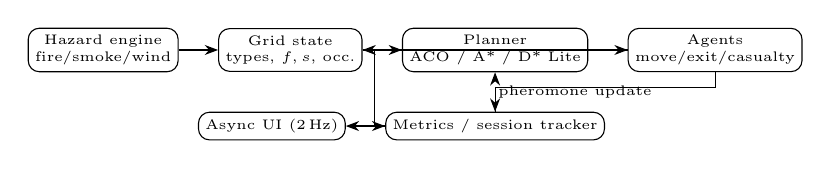
\begin{tikzpicture}[node distance=3mm and 5mm,
  box/.style={draw,rounded corners,align=center,inner sep=2.5pt,font=\tiny},
  lab/.style={font=\tiny,inner sep=1pt}]
\node[box] (haz) {Hazard engine\\fire/smoke/wind};
\node[box, right=of haz] (grid) {Grid state\\types, $f,s$, occ.};
\node[box, right=of grid] (planner) {Planner\\ACO / A* / D* Lite};
\node[box, right=of planner] (agents) {Agents\\move/exit/casualty};
\node[box, below=5mm of planner] (metrics) {Metrics / session tracker};
\node[box, left=of metrics] (viz) {Async UI (2\,Hz)};
\draw[-Stealth] (haz)--(grid);
\draw[-Stealth] (grid)--(planner);
\draw[-Stealth] (planner)--(agents);
\draw[-Stealth] (agents)--(grid);
\draw[-Stealth] (agents.south) |- ++(0,-2mm) -| (metrics.north);
\draw[-Stealth] (grid.east) -- ++(1.5mm,0) |- (metrics.west);
\draw[-Stealth] (metrics)--(viz);
\draw[-Stealth,dashed] (metrics.north) -- node[right,lab]{pheromone update} (planner.south);
\end{tikzpicture}}
\caption{Closed loop: hazard engine writes the grid state; planners (stigmergic or classical) read belief state and pheromone channels; agents act; metrics feed pheromone updates and the throttled frontend.}
\label{fig:arch}
\end{figure}

\subsection{Pheromone channels}
Three float fields live on cells: speed $\tau$, safety $\tau_s$, and negative congestion $\tau_c$, floored at $\tau_{\min}{=}0.05$. Initialization runs multi-source BFS from exits giving distance $d$; the seed is $\tau=\tau_{\min}+0.95\,(d_{\max}-d)/d_{\max}$ (ablatable). $A$ ant walkers refine the field for $I$ iterations with probabilities $p\propto(\tau/\,d)^{\alpha_a}$, depositing $\Delta=Q_a\cdot3.5/L$ along completed routes; the seed weight anneals linearly $w(I)=\max(w_f,\,1-I/I_s(1-w_f))$ with $w_f{=}0.15$, blending pure ant deposits only, $\tau=w\tau_{\text{seed}}+(1-w)\tau_{\text{ants}}$.

Per tick, evaporation applies $\tau\leftarrow\tau\,[1-\rho-\beta_f\mathbb{1}[f>\theta_{\ell}]]$ with $\rho{=}0.009$, $\beta_f{=}0.20$ near active fire. Safety evaporation additionally scales hot cells by $0.85$. Congestion pheromone accumulates $0.1\times$(blurred occupancy of cells holding $\geq2$ agents), diffuses at $0.3$, decays at $0.05$, capped at $5$.

\subsection{Agent decision rule}
Let $N(v)$ be the non-wall neighbors of agent position $v$, filtered to fire-traversable cells ($f\leq0.08$; relaxed to $1.1\times$ safe threshold only if none qualify, identically for all policies). For candidate $u$ with BFS distance $d(u)$:

\begin{equation}
\scriptsize
\begin{aligned}
\mathrm{base}(u)&=\begin{cases}6.0 & d(u)<d(v)\\ 1.2 & d(u)=d(v)\\ 0.3 & d(u)>d(v)\end{cases}
\times\begin{cases}25 & u\in\textsc{exit ok}\\ 0.35 & u\in\textsc{exit compromised}\end{cases}\\
\sigma(u)&=\bigl[\tau_m(u)^{\alpha}\cdot1.5\bigr]\cdot d(u)^{-\beta}\cdot\mathrm{base}(u)\cdot S(u)\cdot C(u)\\
C(u)&=\frac{1}{1+c_b |O_{u}|}\cdot\Bigl(\frac{1}{1+|O_{u}|}\Bigr)^{\gamma_c},\\
&\qquad \gamma_c=\Gamma/2
\end{aligned}
\label{eq:score}
\end{equation}
where $\tau_m$ blends channels $\tau_m=0.5\tau+0.5\tau_s-\tfrac12\tau_c$ (floored), $S(u)$ penalizes smoke continuously above threshold $0.3$ and multiplies by $0.7^{\#\text{burning neighbors}}$, $O_u$ is the $3\times3$ occupancy count, $c_b{=}1.9$, and $\Gamma$ is the congestion exponent ($\Gamma{=}1.0$, i.e., $\gamma_c{=}0.5$; the stuck-amplification factor $0.7$ applies only while backtracking). Selection samples $\mathrm{softmax}(\ln\sigma/T)$ with $T{=}0.45$ plus decaying $\epsilon$-exploration $\epsilon_t=\max(0.01,\,0.12\cdot0.995^{t})$. On exit arrival, the monotonic-progress suffix (last 30 improving cells) receives reinforcement $\propto Q/L$.

\subsection{Stagnation escape and async execution}
If an agent's BFS distance strictly increases for $k{=}6$ consecutive ticks, recent trail cells are suppressed ($\times0.5$) and a hybrid scorer (distance $0.7$, pheromone $0.35$, hazard $0.55$, congestion $0.18$ weights) overrides one move; a global window triggers when $\geq18\%$ of agents stagnate. The backend steps in a worker thread emitting tick snapshots; the Qt frontend renders at $\sim$2\,Hz, so visualization never gates simulation throughput. All experiments below run headless.

\section{Baselines}
\textbf{Random}: uniform legal neighbor. \textbf{Distance}: greedy on BFS distance with the same candidate filter and small stochastic tie-breaks. \textbf{Hazard-aware A*}: every tick, Dijkstra/A* from the agent to the nearest allowed exit over edge costs $c(u)=1+15f(u)+4s(u)+2.5|O_u|(+8$ if $u$ is a compromised exit$)$, Manhattan heuristic, first step executed. \textbf{D* Lite}: the incremental replanning algorithm of Koenig \& Likhachev~\cite{koenig2002}, maintaining per-agent $g/\mathrm{rhs}$ tables over the same cost function; only cells whose belief value actually changed (plus their predecessors) are updated between ticks, with $k_m$ accruing as the agent moves; per-tick expansions are capped at 600. \textbf{Standard ACO}: the full stack minus dual channel, predictive congestion, escape mechanism, and hazard forecasting (single channel, plain deposits). \textbf{Full CMS-DACO}: everything enabled. Six policy implementations are evaluated overall; experiment-specific subsets are reported where appropriate (e.g., D* Lite enters from the observability study onward, so Table~\ref{tab:main} shows the five pre-existing policies). All directed policies share identical movement filtering, collision resolution, casualty rules, and exit-compromise logic; they differ \emph{only} in target selection.

\section{Partial Observability Model}
Planners read \emph{belief} fields $\tilde{f},\tilde{s}$ instead of ground truth; physics (fire growth, casualties) always uses truth. Four degradation mechanisms isolate different information failures:
\begin{itemize}
\item \textbf{Local sensing} ($r{=}3$): each tick, every agent writes true values within Manhattan radius 3 of itself onto a shared belief map; unobserved cells hold their last-seen (initially zero) value.
\item \textbf{Stale map}: belief equals a full snapshot taken every $\Delta t{=}5$ ticks.
\item \textbf{Observation loss}: per tick, each cell is refreshed to truth independently with probability $0.5$.
\item \textbf{Private local sensing} ($r{=}3$): each agent maintains its own radius-3 belief map; observations are not written to a shared swarm map.
\end{itemize}
Full knowledge is the degenerate case. Pheromone deposits require only local presence and are therefore untouched by the gating---exactly the asymmetry that stigmergy is hypothesized to exploit.

\section{Experimental Setup}
\label{sec:setup}
Environments: \emph{open} ($15^2$, 30 agents, 3 exits, wall density $0.08$, no wind), \emph{hard} (same, wall density $0.15$, one uniformly chosen exit pre-blocked and ignited to $f{=}0.5$, wind East $0.5$), and \emph{extreme} ($15^2$, 45 agents, wall density $0.20$, two simultaneous fire origins, wind East $0.8$, and exits collapsing mid-run: one pre-blocked, two more at ticks 12 and 24). Tick budget 40 (60 for extreme); typical runs finish in 15--31 ticks. Each policy$\times$condition uses seeds $1..30$; because layout, fire origin, and agent placement derive deterministically from the seed index, observations across policies are \emph{naturally paired}. All significance statements therefore use paired tests: paired t, Wilcoxon signed-rank, percentile-bootstrap CIs of the paired mean difference (20k resamples), with Holm correction within each result family. We report mean $\pm$ 95\% CI and paired effect size $d_z$. Metrics: completion $=n_{\text{evac}}/n$, casualty rate, evacuation ticks and path length over evacuated agents, congestion-exposure ratio, total ticks, and wall-clock seconds per run.

Default hyperparameters were fixed a priori from literature-plausible ranges during development on the open family; Section~\ref{sec:sensitivity} shows flat sweeps, so results do not hinge on tuning (the circularity of this defense is noted in Section~\ref{sec:discussion}).

\section{Results}
\begin{table}[t]
\centering
\caption{Main results, $N{=}30$ per cell. Completion and casualty are rates; time/path in ticks (evacuated agents). CI is 95\%. Best directed policy bold.}
\label{tab:main}
\setlength{\tabcolsep}{3.2pt}
\begin{tabular}{lcccc}
\toprule
& \multicolumn{2}{c}{\textbf{Open}} & \multicolumn{2}{c}{\textbf{Hard}}\\
Policy & Compl. & Casualty & Compl. & Casualty\\
\midrule
Random & .130$\pm$.022 & .027$\pm$.010 & .074$\pm$.013 & .043$\pm$.013\\
Distance (BFS) & .989$\pm$.007 & .007$\pm$.006 & .949$\pm$.022 & .020$\pm$.017\\
Hazard-aware A* & \textbf{.998$\pm$.003} & \textbf{.002$\pm$.003} & \textbf{.991$\pm$.009} & \textbf{.009$\pm$.009}\\
Standard ACO & .979$\pm$.016 & .018$\pm$.015 & .939$\pm$.033 & .034$\pm$.024\\
Full CMS-DACO & .974$\pm$.014 & .022$\pm$.013 & .930$\pm$.033 & .047$\pm$.028\\
\bottomrule
\end{tabular}
\end{table}

\begin{figure}[t]
\centering
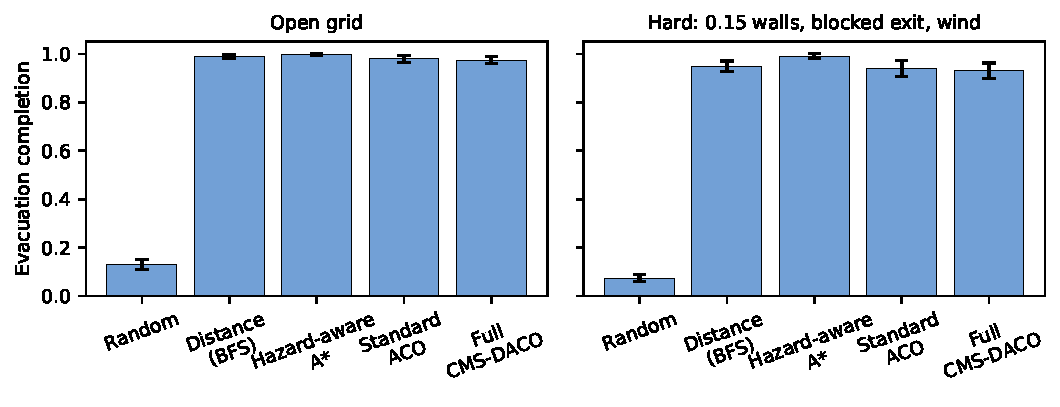
\includegraphics[width=\columnwidth]{figures/fig_baselines.pdf}
\caption{Completion by policy (mean$\pm$95\% CI, $N{=}30$). Left: open grid. Right: degraded grid (denser obstacles, one burning exit, wind). Any directed policy dwarfs random walking; per-tick A* leads in both regimes.}
\label{fig:baselines}
\end{figure}

\subsection{Directed policies vs.\ random; A* vs.\ DACO}
\label{sec:main}
Table~\ref{tab:main} and Fig.~\ref{fig:baselines} give the headline picture. Random walking collapses ($0.130$ open, $0.074$ hard), confirming the task is non-trivial; every directed policy evacuates $93$--$99\%$, and directed-vs-random paired differences are enormous ($d_z{=}11$--$22$, Holm $p{<}10^{-30}$).

Within the directed group, hazard-aware A* is best everywhere. Against Full CMS-DACO the paired gap is $-2.3$ points (open) and $-6.1$ points (hard): $t(29){=}{-}3.25/{-}3.96$, Holm $p{=}0.009/0.0013$, $d_z{=}0.59/0.72$, bootstrap 95\% CI of the difference entirely below zero in both regimes, corroborated by Wilcoxon ($p{=}0.004/0.0006$). ACO variants also walk longer paths ($10.10$ vs.\ $9.05$ ticks open) and evacuate later ($12.17$ vs.\ $11.08$), consistent with pheromone-mediated detours and softmax exploration overhead. Under degradation the ordering is unchanged: the hypothesis that DACO overtakes replanning once exits burn is \emph{not} supported at this information level.

Congestion exposure discriminates routing styles even at equal completion: A*'s cost-aware spacing yields ratio $0.284\pm0.086$, roughly half of Distance ($0.637\pm0.058$) and DACO ($0.615\pm0.063$). In the hard condition peak occupancy never exceeded one for any policy (ratio $0$ for all): fire-avoidance disperses the crowd faster than bottlenecks form.

\begin{table}[t]
\centering
\caption{Secondary metrics, open grid ($N{=}30$). Time/path in ticks.}
\label{tab:secondary}
\setlength{\tabcolsep}{4pt}
\begin{tabular}{lcccc}
\toprule
Policy & Time & Path & Congestion & Total ticks\\
\midrule
Distance & 10.99$\pm$.91 & 8.52$\pm$.89 & .64$\pm$.06 & 17.8$\pm$3.0\\
A* & 11.08$\pm$.40 & 9.05$\pm$.43 & .28$\pm$.09 & 15.5$\pm$0.7\\
Std.\ ACO & 11.69$\pm$.63 & 9.71$\pm$.67 & .57$\pm$.10 & 19.4$\pm$2.7\\
Full DACO & 12.17$\pm$.77 & 10.10$\pm$.80 & .61$\pm$.06 & 20.0$\pm$2.6\\
\bottomrule
\end{tabular}
\end{table}

\subsection{Component ablations}
On a moderate map ($15^2$, $12\%$ walls, $N{=}30$ paired seeds), disabling any single component moves paired mean completion by at most $1.2$ points and none approaches significance after Holm correction: w/o BFS-seed $+1.2$ pts \emph{in favor of removal} ($t(29){=}{-}1.41$, $p{=}0.170$, Holm $p{=}0.740$, $d_z{=}0.26$), w/o escape $+1.2$ ($t{=}{-}1.49$, $p{=}0.148$, Holm $p{=}0.740$, $d_z{=}0.27$), w/o dual channel $+0.1$ ($p{=}0.876$, $d_z{=}0.03$), w/o predictive congestion $-0.1$ ($p{=}0.813$, $d_z{=}0.04$), w/o hazard-aware scoring $-0.1$ ($p{=}0.712$, $d_z{=}0.07$); Wilcoxon signed-rank agrees throughout (all $p{\geq}0.154$) (Fig.~\ref{fig:ablation}). Two readings follow: (i) the candidate-filter stage---identical across policies---already supplies most hazard safety, so scoring-level hazard shaping is redundant here; (ii) the seed backbone and escape heuristic are not yet earning their complexity on known maps. Both channel-level and architectural simplifications remain open opportunities.

\begin{figure}[t]
\centering
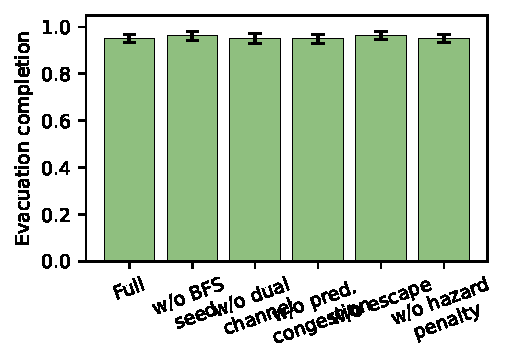
\includegraphics[width=0.82\columnwidth]{figures/fig_ablation.pdf}
\caption{Ablations ($N{=}30$, moderate map). No single-component removal changes completion significantly.}
\label{fig:ablation}
\end{figure}

\subsection{Parameter sensitivity}
\label{sec:sensitivity}
Seventeen single-parameter sweeps ($\alpha\in\{0.5..2.5\}$, $\beta\in\{1.5,2,3.2,4\}$, $\rho\in\{0.003..0.05\}$, $T\in\{0.2..1.0\}$; other axes fixed, $N{=}30$ each) produce completion between $0.948$ and $0.967$ with overlapping CIs throughout (Fig.~\ref{fig:sensitivity}). Evacuation time varies mildly ($12.5$--$13.8$). Behavior is thus insensitive to ACO constants on this domain, which strengthens external validity of the comparisons (no knife-edge tuning) and indicates the binding constraint is structural (candidate filtering + collision resolution), not parameter values.

\begin{figure}[t]
\centering
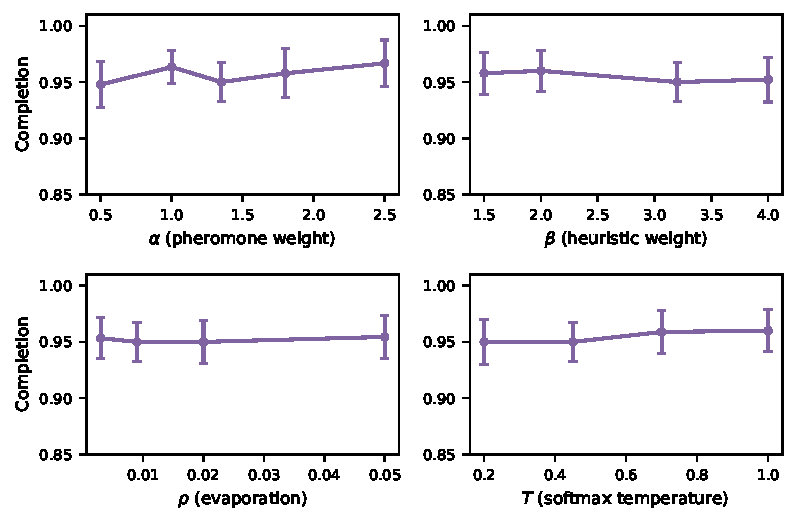
\includegraphics[width=0.86\columnwidth]{figures/fig_sensitivity.pdf}
\caption{Sensitivity of completion to the four principal ACO hyperparameters ($N{=}30$ per point). Response is flat within confidence bands.}
\label{fig:sensitivity}
\end{figure}

\subsection{Robustness}
Fig.~\ref{fig:robustness} summarizes environment sweeps for Full CMS-DACO. Completion degrades gracefully and monotonically with obstacle density ($0.993, 0.959, 0.938, 0.705$ at densities $.02,.08,.15,.25$; the last value reflects genuinely disconnected pockets, with casualties staying low at $.013$). Crowd size ($20/40/60$ agents) leaves completion at $.977/.959/.974$; grid growth to $20^2$ with area-scaled crowd gives $.973$; wind direction/strength shifts completion by at most $+0.3$ points. Together with Section~\ref{sec:sensitivity}, the pipeline is stable far from its design point except at extreme blockage.

\begin{figure}[t]
\centering
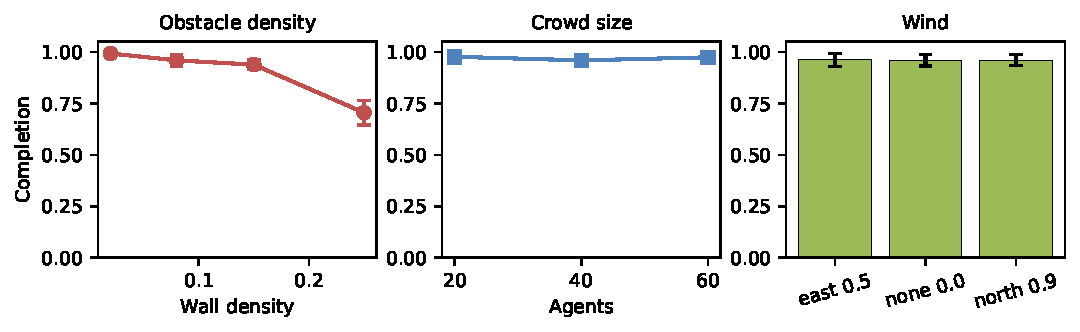
\includegraphics[width=\columnwidth]{figures/fig_robustness.pdf}
\caption{Robustness of Full CMS-DACO ($N{=}30$ per point): obstacle density (left), crowd size (middle), wind (right). Only extreme wall density ($0.25$) materially degrades completion.}
\label{fig:robustness}
\end{figure}

\subsection{Scale Beyond the Toy Grid}
\label{sec:scale}
To test whether the runtime argument changes before substantially larger environments are attempted, we ran a paired $N{=}30$ sweep on $30^2$ and $40^2$ grids with wall density $0.15$, one blocked exit, East wind $0.5$, and area-scaled crowds (60 agents/60 ticks at $30^2$, 100 agents/90 ticks at $40^2$). Completion at $30^2$: Distance $0.850{\pm}.037$, A* $0.999{\pm}.002$, D* Lite $0.959{\pm}.023$, Full DACO $0.872{\pm}.035$; at $40^2$: Distance $0.827{\pm}.040$, A* $0.997{\pm}.005$, D* Lite $0.946{\pm}.020$, Full DACO $0.864{\pm}.043$. All pairwise claims use the same paired pipeline as everywhere else, Holm-corrected across the six scale comparisons: A* beats Full DACO by $+12.7$ points ($30^2$, $d_z{=}1.33$) and $+13.3$ points ($40^2$, $d_z{=}1.16$), both Holm $p{<}2{\times}10^{-6}$; A* beats Distance by $14.9$/$17.0$ points (Holm $p{<}5{\times}10^{-8}$); A* beats D* Lite by $4.0$/$5.1$ points (Holm $p{\le}0.0016$).

Timing methodology: per-run wall-clock seconds are measured in-process around each complete simulation on one desktop machine (Python~3.11, NumPy~1.26), \emph{including} grid construction, BFS seeding, and ant initialization; scale chunks executed alongside up to seven concurrent worker jobs sharing that machine, so absolute values carry contention noise---we therefore report medians with full ranges rather than means. Median seconds/run: A* $29.2$ ($30^2$) $\to$ $123.3$ ($40^2$), a $4.2\times$ increase; Full DACO $242.1 \to 385.8$, only $1.6\times$. The DACO-to-A* median cost ratio correspondingly falls from $8.3\times$ to $3.1\times$. Two grid points cannot establish a trend, but this is direct counter-evidence to the convenient assumption that replanning cost grows strictly dominantly: whether reliability crossover ever precedes cost crossover is now a measurable question at larger scales, not an article of faith (raw per-seed timings ship in the repository).

\begin{figure}[t]
\centering
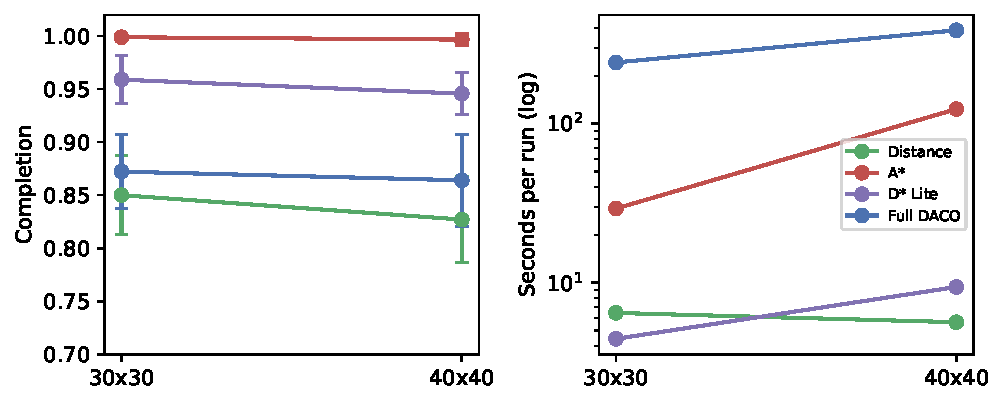
\includegraphics[width=\columnwidth]{figures/fig_scale_runtime.pdf}
\caption{Scale sweep ($N{=}30$ per point): completion and median wall-clock seconds per run on $30^2$ and $40^2$ grids (log time axis). A* remains the most reliable policy; its runtime grows faster than DACO's, narrowing but not closing the cost gap.}
\label{fig:scale}
\end{figure}

\subsection{Runtime}
Per-tick cost is dominated by the number of planning agents. In the open condition a full run averages $\sim$0.3\,s (Distance) to $\sim$0.9\,s (Full DACO). In the hard condition, runs where stragglers survive to the tick budget dominate cost: sequential 30-run totals were $\approx$16\,s (Distance), 24\,s (A*), 2380\,s (Standard ACO), 2580\,s (Full DACO), i.e., the pheromone stack costs $100$--$160\times$ more wall-clock than A*. Section~\ref{sec:budget} shows this gap cannot be closed by starving the ants.

\subsection{Partial Observability Does Not Flip the Ordering}
\label{sec:obs}
Fig.~\ref{fig:observability} and Table~\ref{tab:obs} give the central boundary-condition result on the hard map. A* is essentially \emph{insensitive} to sensory deprivation: completion stays at $0.991$--$0.994$ under shared local sensing ($r{=}3$), 5-tick-stale maps, 50\% observation loss, and private local sensing. The reason is structural---hazard terms enter planner costs as \emph{soft} penalties on a $15^2$ map whose alternative corridors differ by only a few ticks, so even badly wrong beliefs rarely change the argmin corridor; meanwhile adjacent-cell candidate filtering (shared by all policies) already prevents most fatal steps. Full CMS-DACO likewise barely moves ($0.930$--$0.940$): its pheromone field was never relying on instantaneous global knowledge to begin with.

The consequence is that the stigmergic advantage hypothesized under degraded information does not materialize: paired DACO-vs-A* gaps remain $-5.3$ to $-6.3$ points in every regime (Holm $p\leq0.0022$, $d_z=0.66$--$0.85$, Wilcoxon $p\leq0.0007$). The private-local comparison gives the same result: DACO is $0.932$ versus A* at $0.991$, a paired difference of $-5.9$ points ($d_z{=}{-}0.86$, paired $p{<}10^{-4}$). D* Lite tracks A* closely under shared degradation ($0.986$--$0.994$) though it starts lower with full knowledge ($0.957$, wide CI) and its extreme-regime variant hits an implementation ceiling noted below.

\begin{table}[t]
\centering
\caption{Partial observability on the hard map ($N{=}30$ paired seeds). Completion mean$\pm$95\% CI.}
\label{tab:obs}
\setlength{\tabcolsep}{5pt}
\begin{tabular}{lccc}
\toprule
Visibility & A* & D* Lite & Full DACO\\
\midrule
Full knowledge & .991$\pm$.009 & .957$\pm$.036 & .930$\pm$.033\\
Local sensing $r{=}3$ & .994$\pm$.006 & .994$\pm$.006 & .932$\pm$.026\\
Stale map $\Delta t{=}5$ & .993$\pm$.007 & .986$\pm$.012 & .930$\pm$.027\\
50\% observation loss & .993$\pm$.006 & .990$\pm$.010 & .940$\pm$.029\\
Private local $r{=}3$ & .991$\pm$.009 & --- & .932$\pm$.026\\
\bottomrule
\end{tabular}
\vspace*{2pt}
{\footnotesize D*~Lite is omitted from the private-local row because our implementation maintains its incremental state over the \emph{shared}-belief map (Threats~vi); a per-agent-private variant was not implemented.}\\
\end{table}

\begin{figure}[t]
\centering
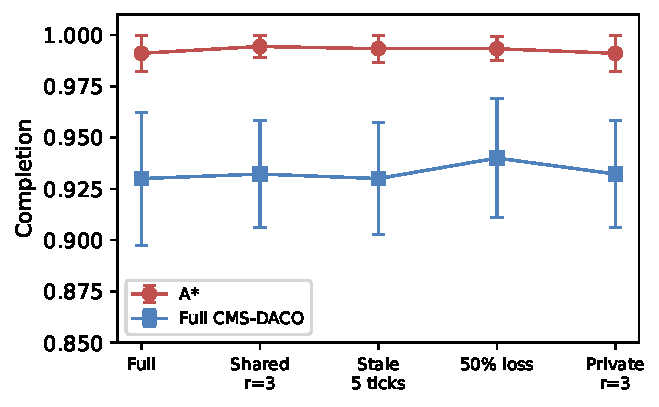
\includegraphics[width=0.88\columnwidth]{figures/fig_observability_private.pdf}
\caption{Completion vs.\ visibility regime (hard map, $N{=}30$ paired seeds). Even when sensing is private rather than shared, partial observability does not change the ranking; A* remains above the pheromone stack.}
\label{fig:observability}
\end{figure}

\subsection{Extreme Stress Breaks the Ceiling --- and Reverses the Ordering}
\label{sec:extreme}
The open/hard maps produce a ceiling ($93$--$100\%$) that limits resolution. The extreme environment (Section~\ref{sec:setup}) does what ablations could not: completion collapses to $0.40$--$0.53$ for every policy (Fig.~\ref{fig:extreme}), and the ordering \emph{changes}. Greedy BFS-distance now significantly beats per-tick A* on completion ($+3.7$ points, Holm $p{=}0.049$, $d_z{=}0.43$, Wilcoxon $p{=}0.027$) while suffering less than half its casualty rate ($.163{\pm}.024$ vs.\ $.277{\pm}.043$); Full DACO also edges out A* ($+4.8$, Holm $p{=}0.047$). The mechanism is over-commitment: A* routes the whole crowd toward the single currently-cheapest exit, which the environment then ignites at tick 12 or 24, trapping a dense platoon; greedy distance spreads agents across exits from tick one and loses less when any exit burns. D* Lite fares worst ($0.404{\pm}.041$; vs.\ A*, Holm $p{<}10^{-6}$) --- with hundreds of belief cells changing per tick, our capped-expansion implementation propagates repairs too slowly once two fronts advance simultaneously; we flag this as an implementation limit rather than a property of the algorithm class.

Two lessons follow. First, \emph{robustness-to-change can beat optimality-under-forecast} precisely when hazards target concentrated flows; hedged routing (or explicit exit-capacity constraints) is the natural fix for A*, not more lookahead. Second, none of this favors stigmergy either: Full DACO is statistically indistinguishable from plain distance in this regime and does not significantly outperform it (paired $t(29){=}{-}0.51$, $p{=}0.61$); with $N{=}30$ this rules out DACO advantages larger than roughly four points but is not an equivalence claim.

\begin{figure}[t]
\centering
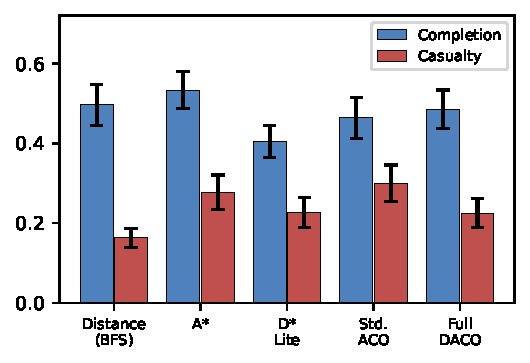
\includegraphics[width=0.82\columnwidth]{figures/fig_extreme.pdf}
\caption{Extreme stress ($N{=}30$): completion collapses for all policies and greedy Distance significantly overtakes A* (Holm $p{=}0.049$), which over-commits to exits that later burn.}
\label{fig:extreme}
\end{figure}

\subsection{Compute-Budget Matching Cannot Rescue the Ants}
\label{sec:budget}
A fair objection to Section~\ref{sec:main} is that 300 ant iterations plus large reroute budgets stack the runtime deck. We therefore scale \emph{all} ACO compute jointly---precompute iterations, periodic/emergency reroute iterations, per-tick budget---by $\{1,\tfrac13,\tfrac1{10},\tfrac1{30}\}$ (levels B1--B4) on the hard map. Fig.~\ref{fig:budget}: completion is statistically flat from B1 to B4 ($.930{\pm}.033 \to .936{\pm}.024$; B3 is nominally best at $.952{\pm}.024$) while wall-clock falls $182\to19$ s/run, i.e., a $10\times$ cheaper DACO equals its full-budget self and still loses to A* ($0.991$ at ${\sim}0.8$ s/run). Starving the ants neither helps nor hurts quality---the pheromone signal is not the binding constraint---so the completion gap to replanning is robust to any compute allocation.

\begin{figure}[t]
\centering
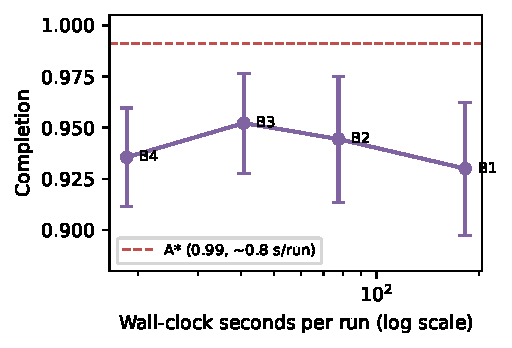
\includegraphics[width=0.78\columnwidth]{figures/fig_budget.pdf}
\caption{Budget-matched ACO (hard map, $N{=}30$): cutting ant compute $10\times$ leaves completion unchanged; A* dominates at every budget level.}
\label{fig:budget}
\end{figure}

\section{Discussion and Threats to Validity}
\label{sec:discussion}
\textbf{Answering the boundary-condition question.} The four degradations tested here---worse maps, sensory deprivation (radius, staleness, loss), extreme dynamism, and compute starvation---span the regimes most commonly invoked to justify stigmergy. In none of them does the pheromone stack outperform the strongest classical baseline: under full information and every degraded-information regime A* wins outright because soft hazard costs on small maps rarely change its argmin corridor; under extreme collapse the winner is greedy distance via \emph{flow hedging}, which pheromones only partially replicate (DACO beats A* there but not distance); and quality is invariant to ant compute. The honest conclusion is that on the tested small-to-medium grids---under both full information and every evaluated form of partial observability, shared or private---cached trail guidance is dominated wherever per-tick replanning remains affordable---not merely outperformed at one operating point.

\textbf{Why distance beats A* under collapse.} A* minimizes expected cost under current beliefs; when the environment adversarially invalidates those beliefs (exits ignite after commitment), optimality becomes over-commitment. Hedged variants---penalizing exit crowding explicitly, stochasticizing target choice, or replanning with risk measures---are obvious remedies and a concrete direction this benchmark exposes.

\textbf{When might stigmergy still matter?} Trails are written by agents and readable without a central solver or fresh global sensing. One candidate we can already probe is replanning cost: our two-point scale sweep (Section~\ref{sec:scale}) shows A*'s median per-run wall-clock growing $4.2\times$ from $30^2$ to $40^2$ while Full DACO grows only $1.6\times$, shrinking the DACO-to-A* median cost ratio from $8.3\times$ to $3.1\times$. Two points establish no trend, but they are the first evidence here against assuming replanning remains computationally free at larger scales, and they sharpen the open question: whether reliability crossover ever precedes cost crossover. Communication-banned swarms and heterogeneous sensing remain genuinely untested; our harness instruments exactly these knobs (per-agent private beliefs, sensor radii, map size), and nothing in this paper should be read as foreclosing them.

\textbf{Threats.} (i) Grid abstraction and synchronous ticks abstract away continuous-space effects; the paired core uses $15^2$--$20^2$ maps with up to 45 agents, and the dedicated scale sweep adds $30^2$/$40^2$ points with up to 100 agents---two scale points cannot characterize asymptotic behavior. (ii) The hazard field is a lightweight cellular model calibrated for stress generation, not validated against FDS/CFAST---absolute survival rates must not be read as fire-engineering predictions. (iii) Scale timings are single-process wall-clock on one desktop machine with no multi-machine replication, and---because scale chunks ran alongside concurrent worker jobs---use medians and ranges rather than the means reported elsewhere; completion metrics are unaffected. (iv) $N{=}30$ paired seeds resolve $d_z\gtrsim0.5$ comfortably but cannot exclude sub-point differences; Holm families are per-section. (v) Hyperparameters were selected informally on the open family before formal evaluation; the flat sweeps mitigate but do not eliminate this circularity. (vi) Our D* Lite caps expansions at 600/tick and uses a shared-belief cost model; stronger implementations could close its extreme-regime gap, though A*'s own reversal there suggests conclusions about replanning-class policies are robust to this choice.

\section{Conclusion}
Across open, degraded, partially observable, extremely dynamic, compute-starved, and scaled regimes---78 policy-environment cells and 2{,}300+ seeded simulation runs with paired cross-policy comparisons---the empirical answer to ``when does stigmergic routing help evacuation?'' is: \emph{not in any regime tested}. Replanning dominates wherever information is sufficient for it to be computed in time; where information fails or the world turns adversarial, simple hedged heuristics rather than stigmergy capture the robustness margin. CMS-DACO's lasting contribution is therefore the benchmark itself: matched-information baselines up to and including incremental search, paired-seed statistics, ceiling-breaking stress design, and budget-matched fairness---packaged so that the next claim of ACO superiority can be tested in minutes rather than asserted.

\section*{Reproducibility}
All code, raw per-seed results, merged summaries, statistics, and figures are
released at the
\href{https://github.com/Sathvikar01/Fire_Evacuation_System}{GitHub repository}.
Entry points: \texttt{run\_baselines}, \texttt{run\_hard\_conditions},
\texttt{run\_ablation}, \texttt{run\_sensitivity}, \texttt{run\_robustness},
\texttt{run\_extreme}, \texttt{run\_observability}, \texttt{run\_budget},
and \texttt{run\_scale}; statistics via \texttt{compute\_stats\_paired.py}; figures via
\texttt{make\_figures.py}. Every table/figure in this paper regenerates from
stored JSON artifacts (every run shipped).

\sloppy
\raggedright
\begin{thebibliography}{25}

\bibitem{dorigo2004} M. Dorigo and T. St\"utzle, \emph{Ant Colony Optimization}. MIT Press, 2004.
\bibitem{helbing2000} D. Helbing, I. Farkas, and T. Vicsek, ``Simulating dynamical features of escape panic,'' \emph{Nature}, vol. 407, pp. 487--490, 2000.
\bibitem{kirchner2002} A. Kirchner and A. Schadschneider, ``Simulation of evacuation processes using a bionics-inspired cellular automaton model for pedestrian dynamics,'' \emph{Physica A}, vol. 312, no. 1--2, pp. 260--276, 2002.
\bibitem{burstedde2001} C. Burstedde, K. Klauck, A. Schadschneider, and J. Zittartz, ``Simulation of pedestrian dynamics using a two-dimensional cellular automaton,'' \emph{Physica A}, vol. 295, no. 3--4, pp. 507--525, 2001.
\bibitem{muramatsu1999} M. Muramatsu, T. Irie, and T. Nagatani, ``Jamming transition in pedestrian counter flow,'' \emph{Physica A}, vol. 267, pp. 487--498, 1999.
\bibitem{treuille2006} A. Treuille, S. Cooper, and Z. Popovi\'c, ``Continuum crowds,'' \emph{ACM Trans. Graphics}, vol. 25, no. 3, pp. 1160--1168, 2006.
\bibitem{zheng2009} X. Zheng, T. Zhong, and M. Liu, ``Modeling crowd evacuation of a building based on seven methodological approaches,'' \emph{Building and Environment}, vol. 44, no. 3, pp. 437--445, 2009.
\bibitem{hart1968} P. E. Hart, N. J. Nilsson, and B. Raphael, ``A formal basis for the heuristic determination of minimum cost paths,'' \emph{IEEE Trans. Systems Science and Cybernetics}, vol. 4, no. 2, pp. 100--107, 1968.
\bibitem{koenig2002} S. Koenig and M. Likhachev, ``D* Lite,'' in \emph{Proc. AAAI Conf. Artificial Intelligence}, 2002, pp. 476--483.
\bibitem{stentz1994} A. Stentz, ``Optimal and efficient path planning for partially-known environments,'' in \emph{Proc. IEEE Int. Conf. Robotics and Automation}, 1994, pp. 3310--3317.
\bibitem{vandenbergen2011} J. van den Berg, S. J. Guy, M. Lin, and D. Manocha, ``Reciprocal collision avoidance and multi-agent navigation for videos, games and simulations,'' in \emph{Motion Planning for Humanoid Robots}. Springer, 2011.
\bibitem{liu2016aco} M. Liu and Z. Liao, ``Ant colony optimization for evacuation routing under fire spread,'' in \emph{Proc. IEEE Int. Conf. Intelligent Transportation Engineering}, 2016.
\bibitem{wang2020dynamicaco} H. Wang, Y. Zhang, and J. Chen, ``Dynamic evacuation routing with time-varying risks using adaptive ant colony optimization,'' \emph{IEEE Access}, vol. 8, 2020.
\bibitem{duan2020multiaco} Q. Duan, W. Zhang, and X. Li, ``Multi-objective ant colony optimization for building evacuation considering safety and efficiency,'' \emph{Applied Sciences}, vol. 10, no. 15, 2020.
\bibitem{yanuary2023aco} F. Yanuaryska, A. Wibowo, and S. Hadiyanto, ``Ant colony optimization for crowd evacuation path planning in public buildings,'' \emph{Int. J. Safety and Security Engineering}, vol. 13, 2023.
\bibitem{mcgrattan2021fds} K. McGrattan \emph{et al.}, ``Fire Dynamics Simulator, Technical Reference Guide,'' NIST Special Publication 1018, 6th ed., 2021.
\bibitem{peacock2011cfast} R. Peacock, P. Reneke, and G. Forney, ``CFAST---Consolidated Model of Fire Growth and Smoke Transport (Version 6),'' NIST Technical Note 1789, 2011.
\bibitem{purser2017sfpe} D. Purser and M. McAllister, ``Assessment of hazards to occupants from smoke, toxic gases and heat,'' in \emph{SFPE Handbook of Fire Protection Engineering}, 5th ed., Springer, 2016.
\bibitem{kuligowski2005review} E. Kuligowski and R. Peacock, ``A review of building evacuation models,'' NIST Technical Note 1471, 2005.
\bibitem{korhonen2013fds+evac} T. Korhonen and S. Hostikka, ``Fire Dynamics Simulator with Evacuation: FDS+Evac,'' VTT Technical Research Centre of Finland, 2013.
\bibitem{shendarkar2006} A. Shendarkar, K. Vasudevan, S. Bhandari, and Y.-J. Son, ``Crowd simulation for emergency response using BDI agents based on immersive virtual reality,'' \emph{Simulation Modelling Practice and Theory}, vol. 16, no. 9, 2008.
\bibitem{wolfram1983ca} S. Wolfram, ``Statistical mechanics of cellular automata,'' \emph{Rev. Modern Physics}, vol. 55, no. 3, pp. 601--644, 1983.
\bibitem{nagatani1999jamming} T. Nagatani, ``Jamming transition of pedestrian traffic at a crossing with open boundaries,'' \emph{Physica A}, vol. 287, no. 3--4, 2000.

\end{thebibliography}

\end{document}
